\documentclass[aspectratio=169]{beamer}

\usetheme{metropolis}

\usepackage[spanish]{babel}
\usepackage[utf8]{inputenc}
\usepackage{amsmath,amssymb}
\usepackage{graphicx}
\usepackage{booktabs}
\usepackage{xcolor}

% Paquete para citas en pie de página
\usepackage[natbib=true, style=authoryear, backend=biber]{biblatex}
\addbibresource{referencias.bib}
\setbeamercolor{background canvas}{bg=white}
% Comando para cita completa en pie de página
\newcommand{\fullfootcite}[1]{%
    \footcite[#1]{#1}%
}

% Comandos útiles
\newcommand{\ket}[1]{\lvert #1 \rangle}
\newcommand{\bra}[1]{\langle #1 \rvert}
\newcommand{\braket}[2]{\langle #1 | #2 \rangle}

\title{Trayectorias Cuánticas para simular Fluorescencia Resonante}
\subtitle{Óptica Cuántica}
\author{Kevin Martínez Franco}
\institute{
    Universidad Autónoma del Estado de Morelos \\
    Centro de Investigación en Ingeniería y Ciencias Aplicadas
}
\date{8 de diciembre de 2025}

\begin{document}

\maketitle

\begin{frame}{Índice}
\tableofcontents
\end{frame}

%------------------------------------------------
\section{Sistemas Cuánticos Abiertos}
\note{
\textbf{Contexto general:}
En óptica cuántica, trabajamos principalmente con Sistemas Cuánticos Abiertos (SQA). Esto se debe a que en la práctica, ningún sistema está perfectamente aislado. 

\textbf{Relevancia:}
Esta presentación se centra en fluorescencia atómica resonante, que es uno de los fenómenos más importantes en óptica cuántica. La fluorescencia ocurre cuando un átomo excitado emite fotones al decaer a su estado fundamental.

\textbf{Emisión espontánea:}
La emisión espontánea es un proceso fundamental que no puede describirse con mecánica cuántica estándar de sistemas cerrados. Por eso necesitamos el formalismo de SQA.

\textbf{Importancia práctica:}
Entender estos sistemas es crucial para:
- Relojes atómicos
- Computación cuántica
- Espectroscopia de alta precisión
- Generación de estados no clásicos de luz
}


\begin{frame}{Introducción: Sistemas Cuánticos Abiertos}

El acoplamiento de un átomo a un entorno con una gran cantidad de modos del campo electromagnético provoca emisión espontánea. El sistema transfiere irreversiblemente energía al entorno (los modos del vacío cuántico). El anterior fenómeno es una manifestación de la disipación.
\vspace{-0.3cm}

\centering
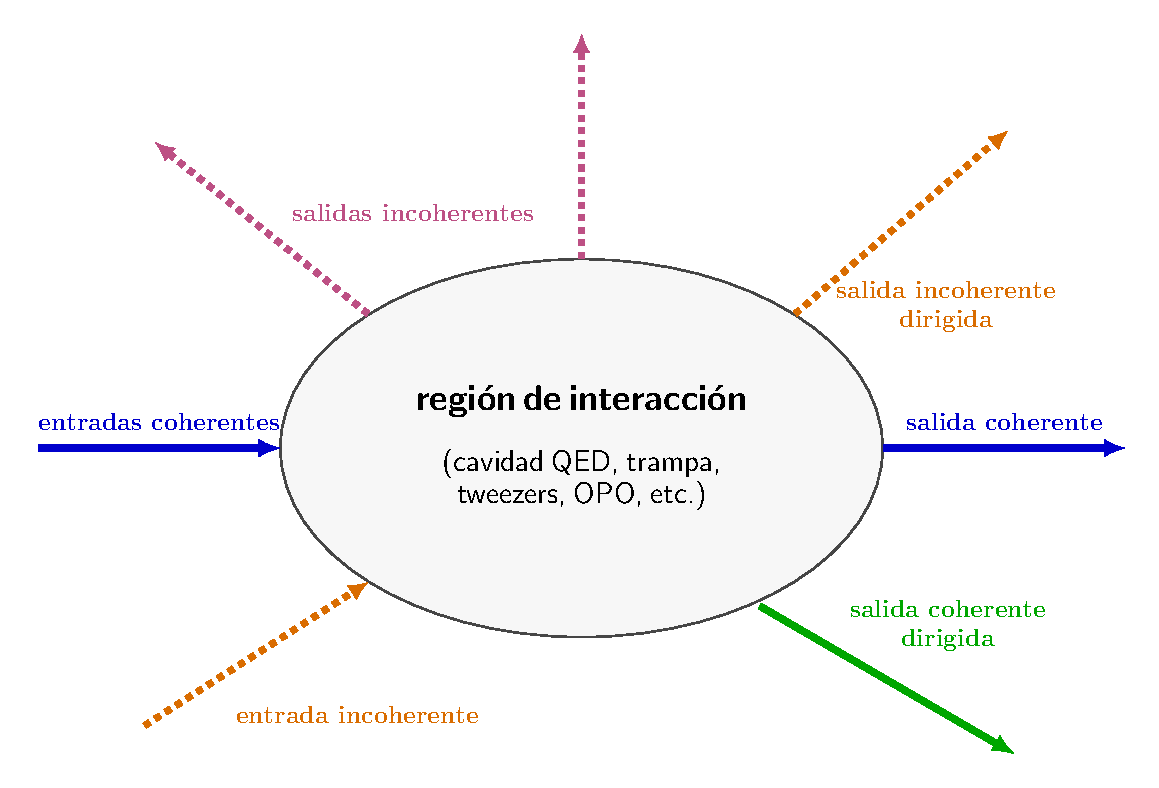
\includegraphics[width=0.55\textwidth]{imagenes/SQA.pdf}


\end{frame}

\begin{frame}{Ecuación Maestra}

\begin{block}{Descripción}
Describe la \textbf{dinámica promedio} de un ensamble utilizando un \textbf{operador de densidad} que describe un estado mixto.
\end{block}

\vspace{0.2cm}

El operador densidad para un estado puro se define como:
\[
\rho = \ket{\Psi}\bra{\Psi}
\]

\vspace{0.2cm}

Su evolución temporal está dada por la ecuación maestra de Lindblad:
\[
\boxed{\frac{\partial \rho}{\partial t} = -\frac{i}{\hbar} \left[ H, \rho \right] + \mathcal{D}[\rho]}
\]

\vspace{0.2cm}

donde:
\begin{itemize}
\item $\rho$ es el operador de densidad del sistema
\item $H$ es el Hamiltoniano del sistema
\item $\mathcal{D}[\rho] = \sum_k \gamma_k \left( L_k \rho L_k^\dagger - \frac{1}{2} \{L_k^\dagger L_k, \rho\} \right)$ es el disipador de Lindblad
\end{itemize}

\end{frame}

%------------------------------------------------
\section{Trayectorias Cuánticas}

\begin{frame}{Trayectorias Cuánticas}
\begin{block}{Idea central}
Descomponen la dinámica de $\rho (t)$ en evoluciones estocástica de estados puros $|\psi(t)\rangle$.
\end{block}

\begin{itemize}
\item Cada trayectoria representa una posible historia del sistema bajo \textbf{detección continua} del entorno.

\end{itemize}

\vspace{0.3cm}
\begin{center}
    Las trayectorias Cuánticas pueden ser \textbf{Discontinuas} y \textbf{Difusivas}
\end{center}
.
\end{frame}
\begin{frame}{Convergencia del método de trayectorias cuánticas discontinuas}

\begin{columns}
\column{0.4\textwidth}

\begin{equation}
 \bar{\rho}(t)= \frac{1}{N} \sum_{k=1}^{N} \rho_k(t)   
\end{equation}




\begin{equation}
\epsilon \propto \frac{1}{\sqrt{N}}
\end{equation}








\end{columns}

\end{frame}


\section{Fluorescencia Resonante Intermitente}

\begin{frame}{Fluorescencia Resonante Intermitente}
\begin{columns}[T]

\column{0.5\textwidth}
Es la fluorescencia atómica donde ocurren aleatoriamente periodos \textbf{brillantes} y \textbf{oscuros}.\\
Estudiarla es especialmente útil para entender transiciones débiles.

\vspace{0.5cm}
\centering
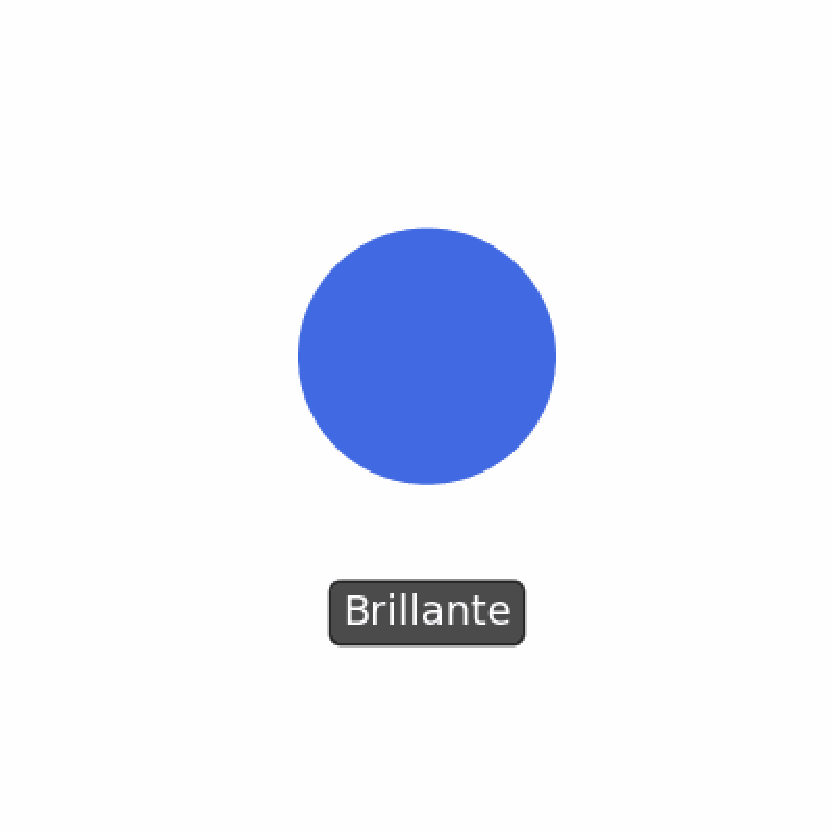
\includegraphics[width=0.8\textwidth]{imagenes/gifFRI.pdf} % PDF con múltiples páginas

\column{0.5\textwidth}
\centering
\begin{figure}
\caption{Esquema del sistema de 3 niveles}
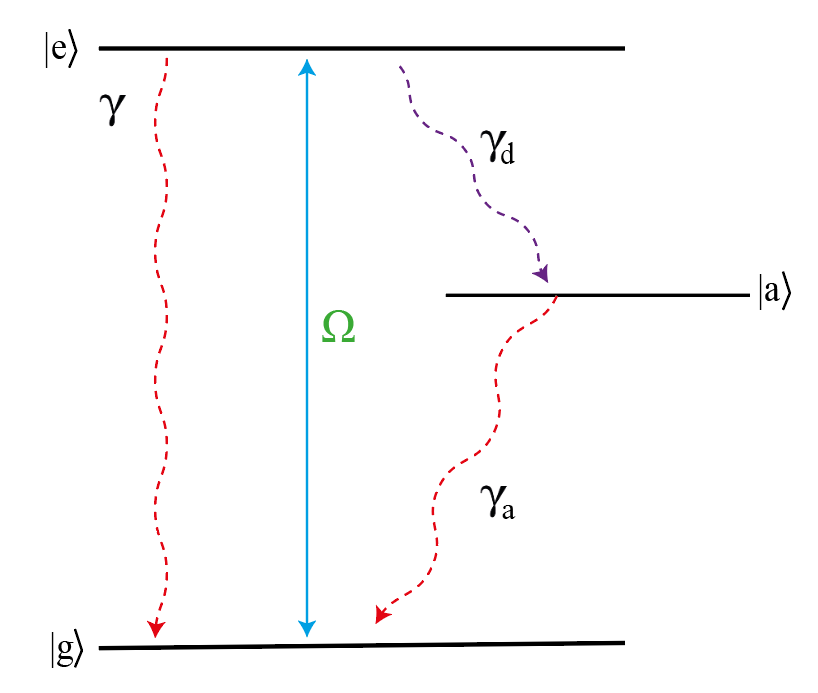
\includegraphics[width=0.7\textwidth]{imagenes/1 sistema.png}
\end{figure}
$\gamma >> \gamma_d, \gamma_a$
\end{columns}
\end{frame}




%------------------------------------------------
\section{Herramientas Computacionales}

\begin{frame}{Herramientas para Simular SCA}

\begin{itemize}
\item Python orientado a objetos.
\item NumPy y SciPy.
\item Matplotlib.
\item QuTiP.
\end{itemize}

\vspace{0.5cm}

\begin{block}{Solvers utilizados}
\begin{itemize}
\item Lindblad Master Equation Solver.
\item Monte Carlo Solver.
\item Stochastic Solver.
\end{itemize}
\end{block}
\end{frame}

%------------------------------------------------
\section{Trayectorias Discontinuas}

\begin{frame}{Trayectorias Discontinuas}
\begin{itemize}
\item Evolución no unitaria entre saltos.
\item Saltos cuánticos asociados a emisiones detectadas.
\item Método equivalente a la ecuación maestra tras promediar muchas trayectorias.
\end{itemize}

\vspace{0.5cm}

\begin{block}{Ecuación de Schrödinger estocástica}
\[
d\ket{\psi(t)} = \left[ - \frac{i}{\hbar} H_{\text{eff}} \, dt + \sum_k \left( \frac{L_k}{\sqrt{\langle L_k^\dagger L_k \rangle}} - 1 \right) dN_k \right] \ket{\psi(t)}
\]
donde $H_{\text{eff}} = H - \frac{i\hbar}{2} \sum_k L_k^\dagger L_k$ es el Hamiltoniano efectivo.
y $ H =
\Delta \sigma_{ee}
+
\frac{\Omega}{2}
\left(
\sigma_{eg}+\sigma_{ge}
\right)
$
\end{block}
\end{frame}

\begin{frame}{Periodos Brillantes y Oscuros}

\begin{columns}[T]

\column{0.48\textwidth}
\centering
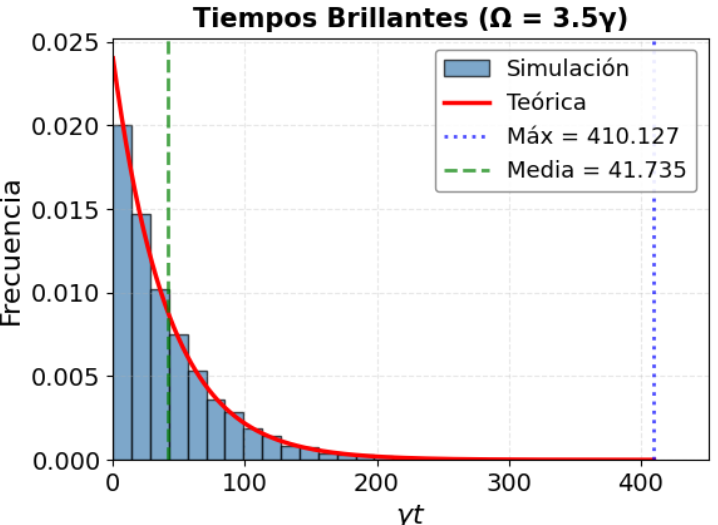
\includegraphics[width=\textwidth]{imagenes/TB.png}
\vspace{0.2cm}

{\small Periodos Brillantes}

\column{0.48\textwidth}
\centering
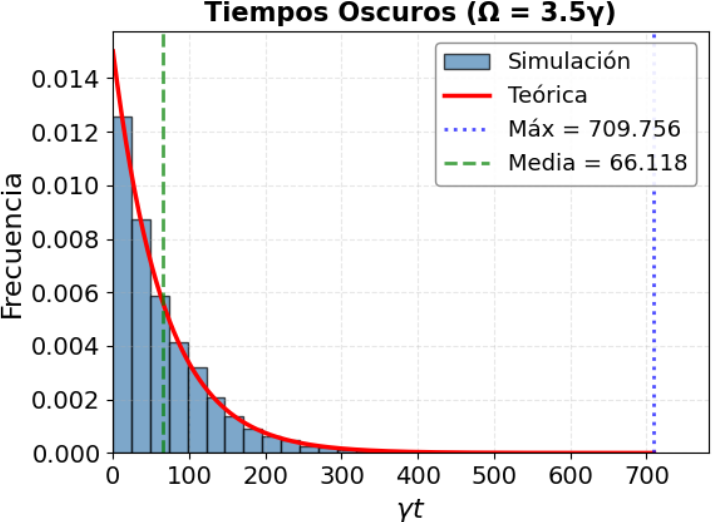
\includegraphics[width=\textwidth]{imagenes/TO.png}
\vspace{0.2cm}

{\small Periodos Oscuros}

\end{columns}

\vspace{0.3cm}

\centering
{\small $\Omega = 3.5\gamma$}

\end{frame}

\begin{frame}{Distribución de tiempos de espera}
    \begin{center}
    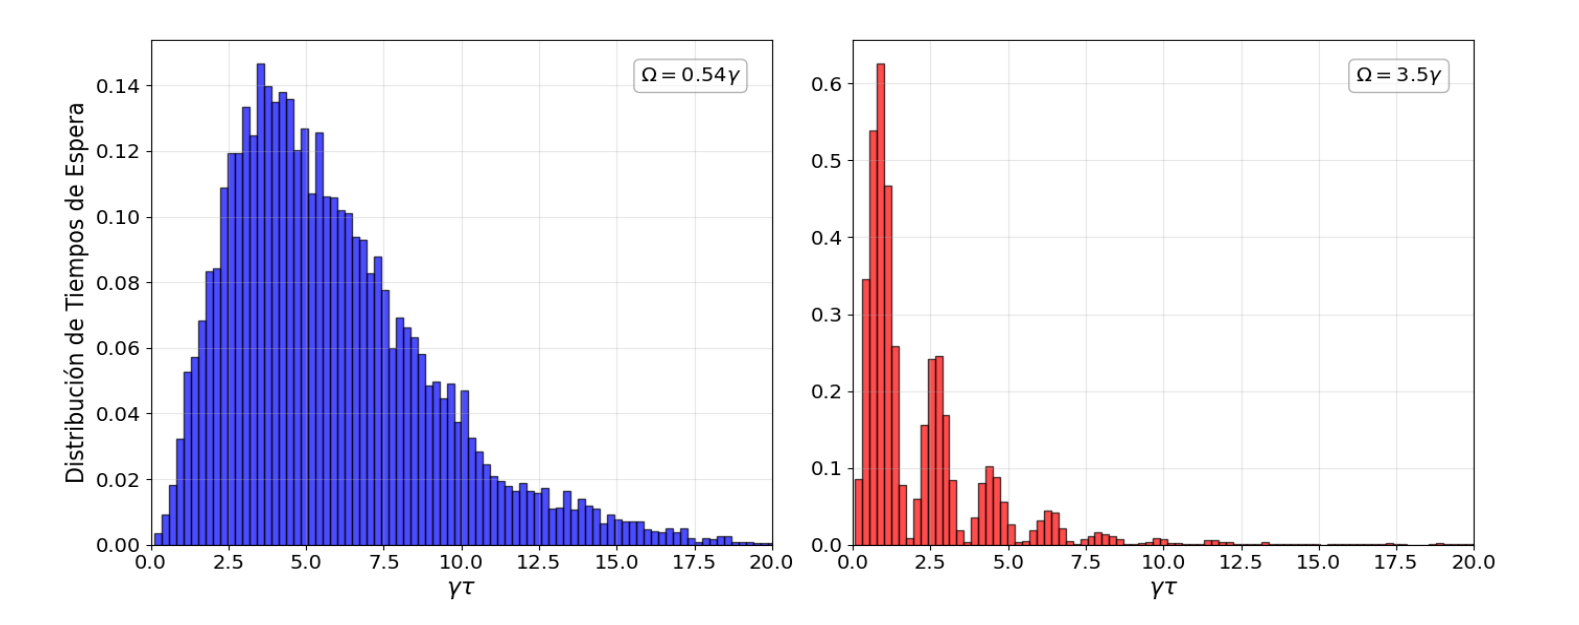
\includegraphics[width=1\textwidth]{imagenes/tiespera.png}
    \end{center}
\end{frame}

%------------------------------------------------
\section{Detección Homodina y Heterodina}

\begin{frame}{Detección Homodina y Heterodina}

\begin{columns}[T]

\column{0.55\textwidth}
\begin{itemize}
\item El campo emitido se mezcla con un oscilador local.
\item Se emplea un divisor de haz.
\item La diferencia de fotocorrientes contiene información espectral.
\end{itemize}

\column{0.45\textwidth}
\centering
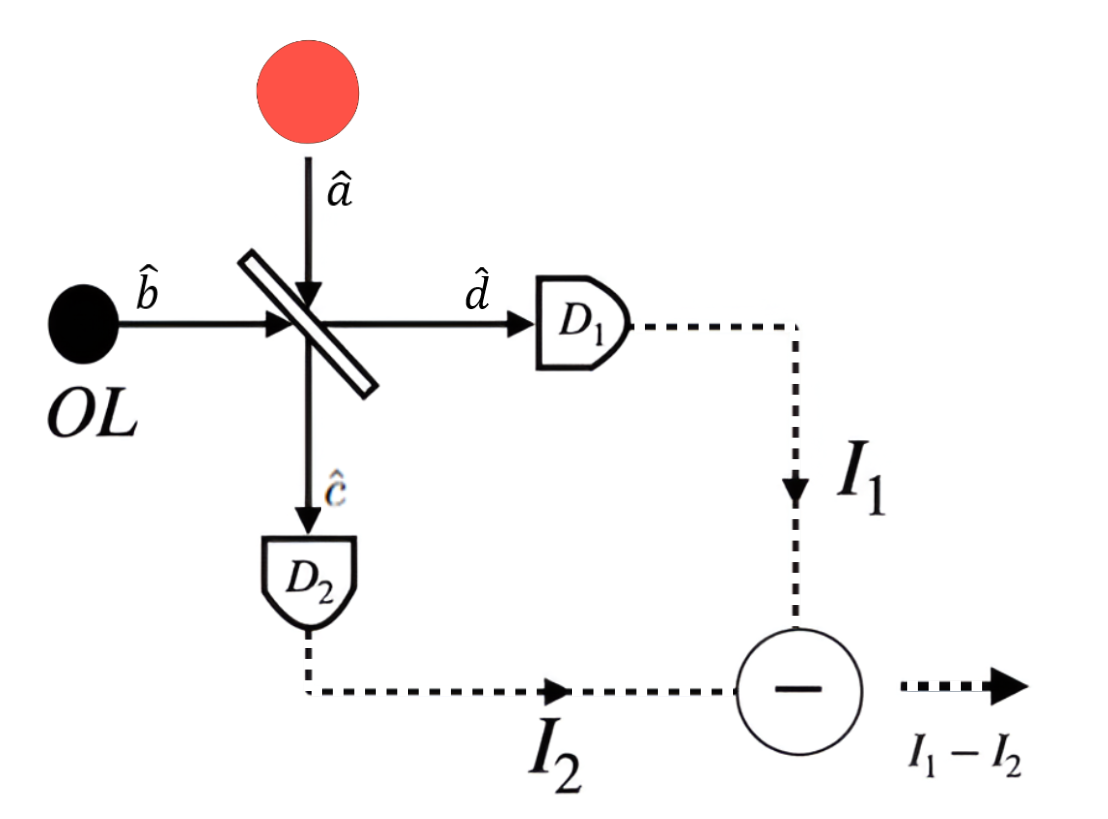
\includegraphics[width=\textwidth]{imagenes/dhb.png}

\end{columns}
\end{frame}

%------------------------------------------------
\section{Trayectorias Difusivas}

\begin{frame}{Trayectorias Difusivas Heterodinas}

\begin{itemize}
\item Basadas en una medición continua del campo emitido.
\item Incorporan ruido complejo de Wiener.
\item Generan una fotocorriente estocástica.
\end{itemize}

\vspace{0.5cm}

\begin{block}{Ecuación de evolución estocástica heterodina}
\[
d\ket{\tilde{\psi}} = \left[ - \frac{i}{\hbar} H_{\text{eff}} \, dt + \sqrt{\gamma} \left( \langle \sigma_- \rangle_{\tilde{\psi}} \, dt + \frac{dW}{\sqrt{2}} \right) (\sigma_- - \langle \sigma_- \rangle_{\tilde{\psi}}) \right] \ket{\tilde{\psi}}
\]
con ruido complejo $dW = (dW_1 + i dW_2)/\sqrt{2}$.

\end{block}
\end{frame}



\begin{frame}{Fotocorriente Heterodina}

\centering
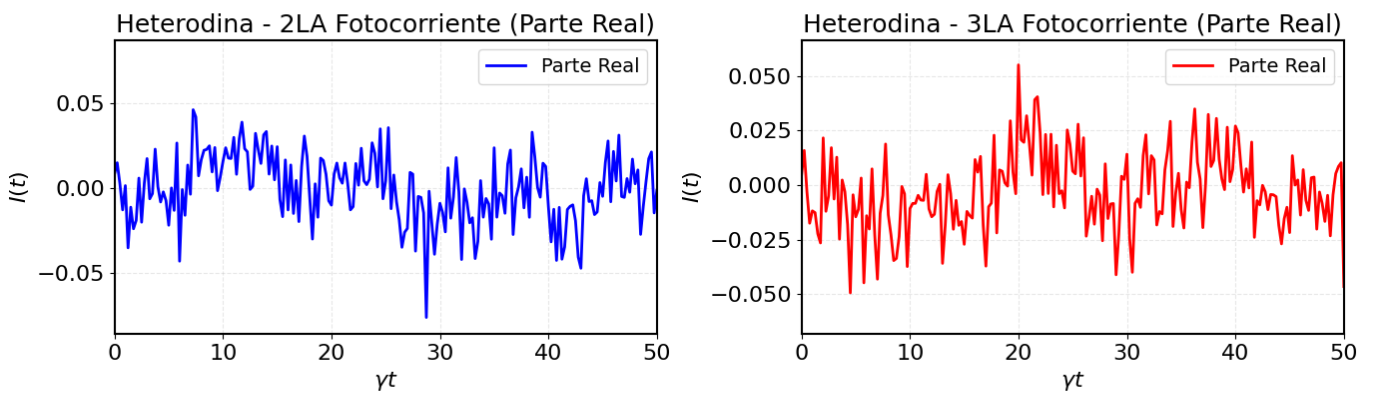
\includegraphics[width=1\textwidth]{imagenes/fotocorrientehetero.png}

\end{frame}

\begin{frame}{Autocorrelación}

\centering
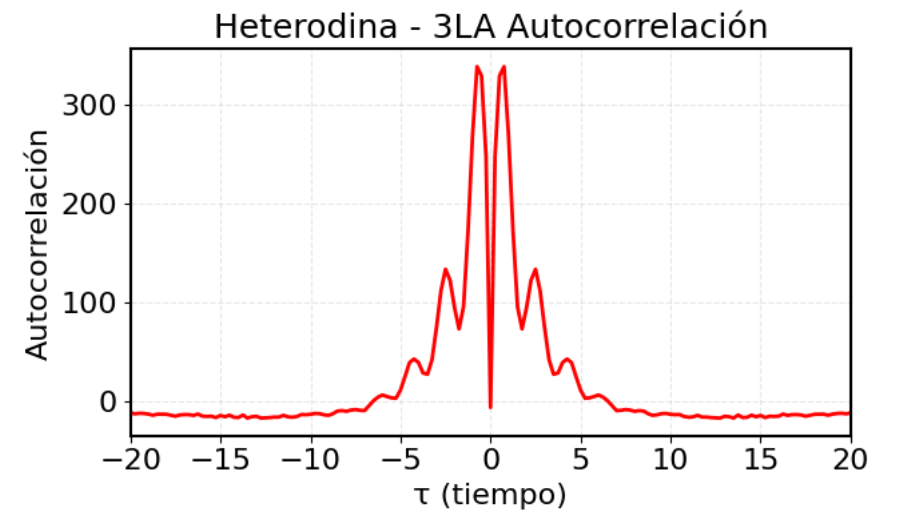
\includegraphics[width=0.7\textwidth]{imagenes/autocorrelacionhetero.png}

\end{frame}

\begin{frame}{Espectro Heterodino: Triplete de Mollow}

\centering
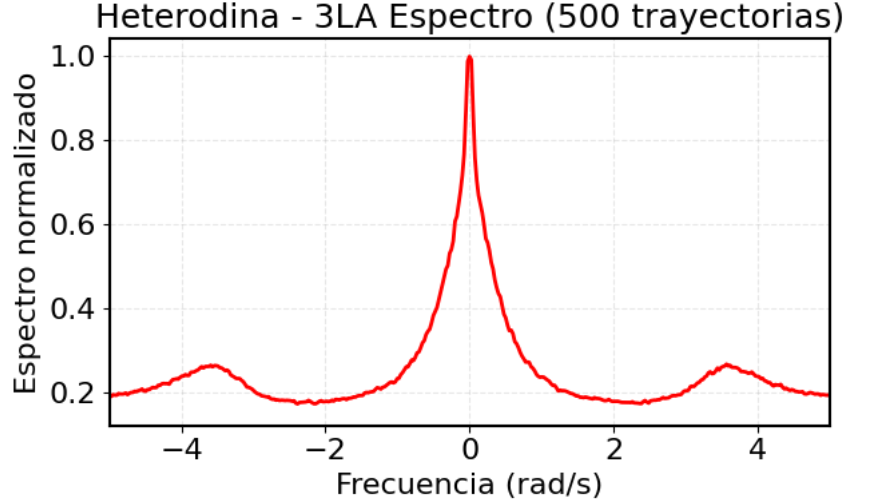
\includegraphics[width=0.7\textwidth]{imagenes/heterodinamollow35.png}

\end{frame}

\begin{frame}{Frecuencia de Rabi Óptima}

\centering
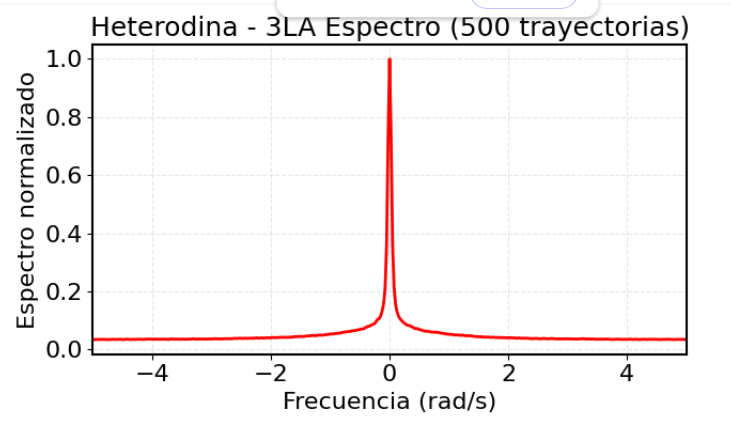
\includegraphics[width=0.7\textwidth]{imagenes/heterodinaopt054.png}

\end{frame}

%------------------------------------------------
%------------------------------------------------
%------------------------------------------------
\section{Dinámica del Estado Cuántico}

\begin{frame}{Dinámica del Átomo de Dos Niveles}

\centering
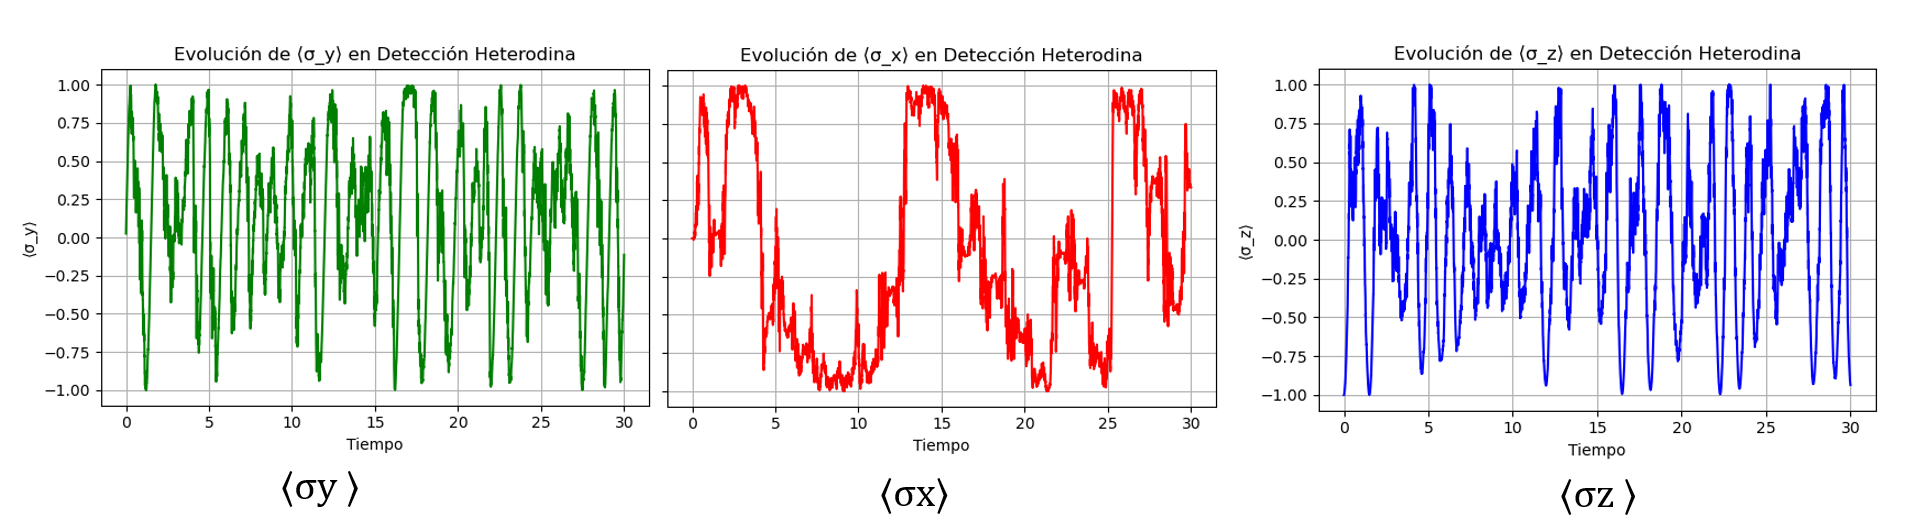
\includegraphics[width=0.8\textwidth]{imagenes/sigmatime.png}




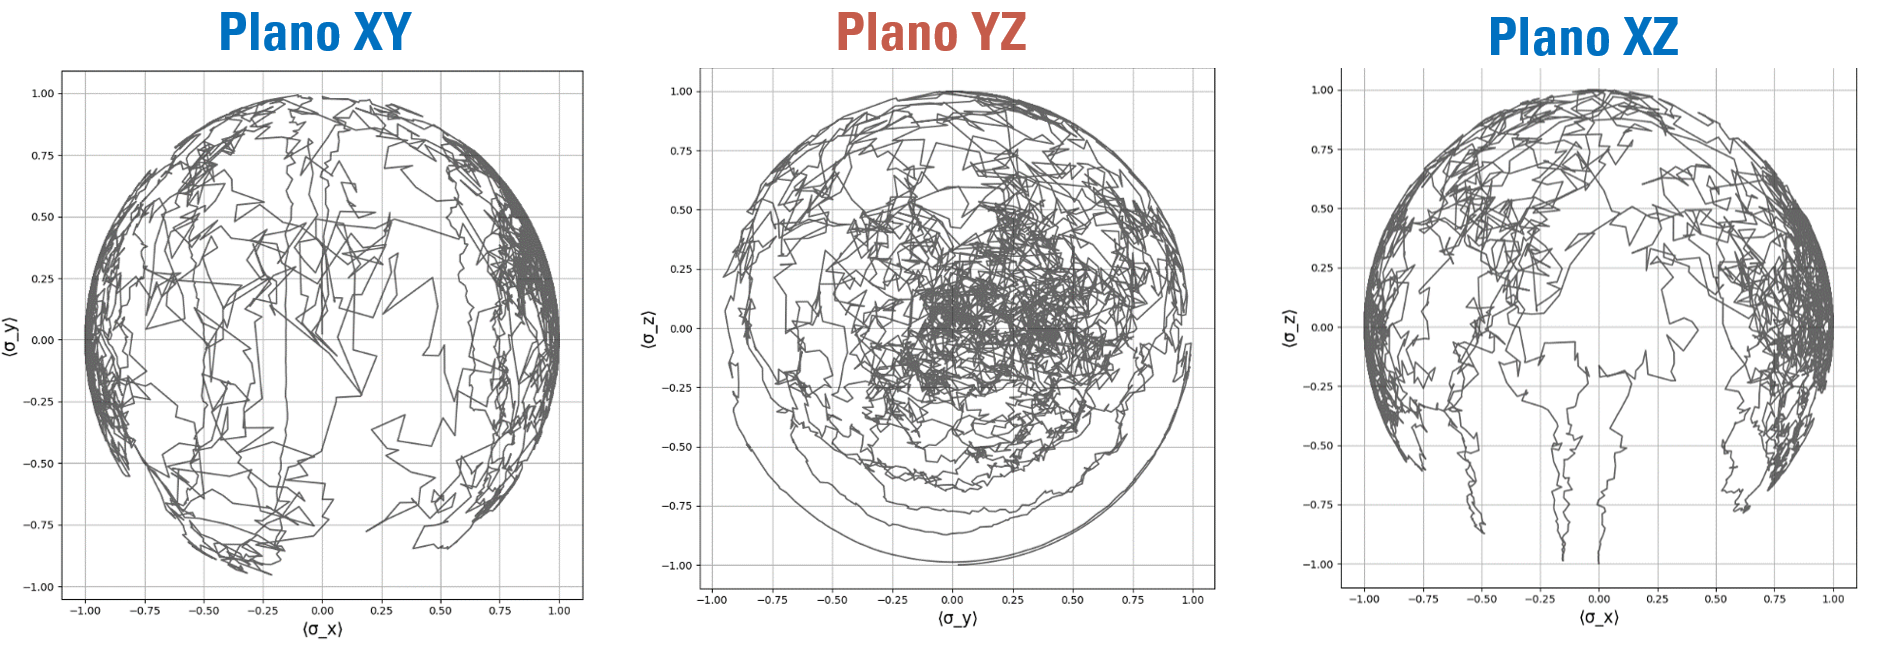
\includegraphics[width=0.8\textwidth]{imagenes/simgaplanos.png}


{\small \textbf{(b)} Trayectoria en la esfera de Bloch}

\note{
\textbf{Contexto:}
- Esta diapositiva muestra la dinámica de un átomo de dos niveles bajo una trayectoria cuántica difusiva.
- Es el resultado de una simulación de Monte Carlo de la ecuación maestra.

\textbf{Gráfica (a) - Evolución temporal de σₓ:}
- En la parte superior vemos la evolución temporal del valor esperado de $\sigma_x$.
- Observamos un comportamiento de \textit{switching} o conmutación.
- El sistema alterna entre valores cercanos a +1 y -1.
- Estos saltos corresponden a cambios abruptos en el estado cuántico.
- Los saltos ocurren en tiempos aleatorios.

\textbf{¿Qué es el switching y por qué ocurre?}
- El switching es un fenómeno donde el sistema salta entre dos estados metaestables.
- En este caso, el átomo conmuta entre dos cuadraturas del campo.
- Esto es característico de las trayectorias cuánticas difusivas.
- La medición continua proyecta el sistema a estados con fase definida.
- Cada salto corresponde a un evento de detección.

\textbf{Gráfica (b) - Esfera de Bloch:}
- En la parte inferior vemos la trayectoria en la esfera de Bloch.
- La esfera de Bloch es una representación geométrica del estado de un qubit.
- Cada punto en la esfera representa un estado cuántico puro.
- La trayectoria muestra cómo evoluciona el estado condicionado.
- El estado se mueve principalmente cerca del ecuador de la esfera.

\textbf{Interpretación física:}
- El switching en $\sigma_x$ indica que la fase del campo emitido cambia.
- Esto está relacionado con la detección homodina/heterodina.
- Las mediciones continuas proyectan el sistema a estados con fase definida.
- $\sigma_x$ mide la coherencia entre los niveles atómicos.

\textbf{Importancia del resultado:}
- Este comportamiento no se ve en la dinámica promedio (ecuación maestra).
- Es una manifestación del condicionamiento por la medición.
- Muestra que las trayectorias individuales contienen más información.
- Es crucial para entender la física de sistemas cuánticos abiertos.
- Demuestra que el acto de medir afecta la evolución del sistema.

\textbf{Aplicaciones prácticas:}
- Entender este switching es importante para:
  * Control de estados cuánticos en tiempo real
  * Metrología cuántica y mediciones de alta precisión
  * Procesamiento de información cuántica
  * Simulación de sistemas cuánticos abiertos

\textbf{Conexión con la teoría:}
- Este resultado confirma las predicciones teóricas de las trayectorias cuánticas.
- Muestra la equivalencia entre el formalismo de Monte Carlo y la ecuación maestra.
- El promedio sobre muchas trayectorias reproduce el resultado de la ecuación maestra.

\textbf{Transición a lo siguiente:}
"Ahora que hemos visto la dinámica del estado cuántico y el switching en σₓ, pasaremos a analizar los espectros de fluorescencia que resultan de estas trayectorias."
}

\end{frame}



%------------------------------------------------
\section{Trayectorias Difusivas Homodinas}

\begin{frame}{Trayectorias Difusivas Homodinas}

\begin{itemize}
\item La medición selecciona una cuadratura del campo.
\item La fase $\phi$ determina la cuadratura observada.
\item La dinámica depende explícitamente de la fotocorriente medida.
\end{itemize}

\vspace{0.5cm}

\begin{block}{Ecuación de evolución estocástica homodina}
\[
d\ket{\psi} = \left[ - \frac{i}{\hbar} H_{\text{ef}} \, dt + \sqrt{\gamma} \left( \langle \sigma_- e^{i\phi} + \sigma_+ e^{-i\phi} \rangle_{\psi} \, dt + dW \right) (\sigma_- e^{i\phi} - \langle \sigma_- e^{i\phi} \rangle_{\psi}) \right] \ket{\psi}
\]
donde $dW$ es ruido real de Wiener.
\end{block}
\end{frame}

\begin{frame}{Espectros Homodinos}

\begin{columns}[T]

\column{0.5\textwidth}
\centering
$\phi = 0$ \\
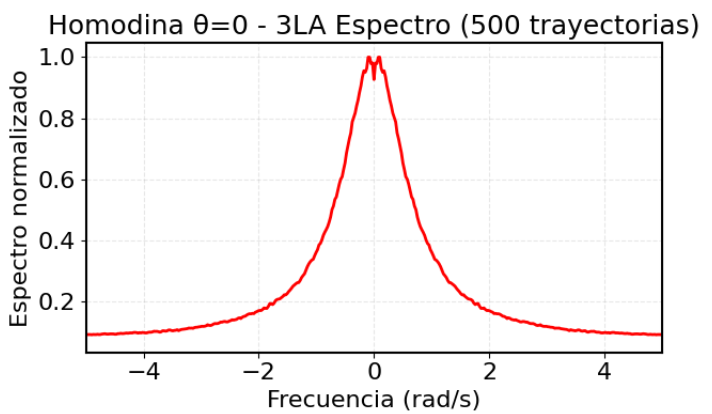
\includegraphics[width=\textwidth]{imagenes/homodina035.png}

\column{0.5\textwidth}
\centering
$\phi = \pi/2$ \\
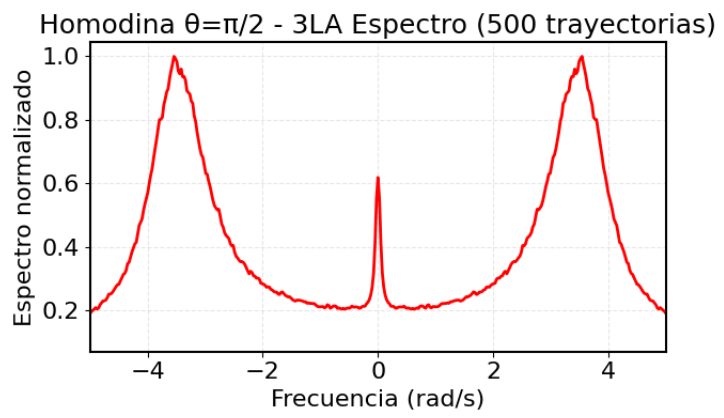
\includegraphics[width=\textwidth]{imagenes/homodinapi34.png}

\end{columns}
\end{frame}

%------------------------------------------------
\section{Conclusiones}

\begin{frame}{Conclusiones}

\begin{itemize}
\item Se estudiaron trayectorias cuánticas discontinuas y difusivas.
\item Se reprodujeron características fundamentales de la fluorescencia resonante intermitente.
\item Se obtuvieron espectros heterodinos y homodinos.
\item Las trayectorias permiten interpretar la dinámica condicionada del sistema.
\end{itemize}

\vspace{0.3cm}

\textbf{Aplicaciones}

\begin{itemize}
\item Relojes atómicos ópticos.
\item Espectroscopia de alta resolución.
\item Microscopía de fluorescencia.
\end{itemize}
\end{frame}

%------------------------------------------------
\begin{frame}[allowframebreaks]{Referencias}

\begin{thebibliography}{9}
\begin{itemize}
    \item H. J. Carmichael, \textit{An Open Systems Approach to Quantum Optics}, Springer, Berlin, 1993.

    \item H. J. Carmichael, in \textit{Coherence and Quantum Optics VII}, Springer, Boston, MA, 1993.

    \item H. M. Wiseman and G. J. Milburn, \textit{Phys. Rev. A} \textbf{47}, 1652 (1993).

    \item H. M. Wiseman and G. J. Milburn, \textit{Quantum Measurement and Control}, Cambridge University Press, Cambridge, 2010.

    \item J. T. Höffges, H. W. Baldauf, T. Eichler, S. R. Helmfrid, and H. Walther, \textit{Opt. Commun.} \textbf{133}, 170 (1997).

    \item J. T. Höffges, H. W. Baldauf, W. Lange, and H. Walther, \textit{J. Mod. Opt.} \textbf{44}, 1099 (1997).

    \item M. B. Plenio and P. L. Knight, \textit{Rev. Mod. Phys.} \textbf{70}, 101 (1998).

    \item V. Bühner and Ch. Tamm, \textit{Phys. Rev. A} \textbf{61}, 061801 (2000).

    \item R. Román-Ancheyta, O. de los Santos-Sánchez, L. Horvath, and H. M. Castro-Beltrán, ``Time-dependent spectra of a three-level atom in the presence of electron shelving'', \textit{Phys. Rev. A} \textbf{98}, 013820 (2018).

    \item M. O. Scully and M. S. Zubairy, \textit{Quantum Optics}, Cambridge University Press, Cambridge, 1997, p.~125.

    \item R. M. Godun, P. B. R. Nisbet-Jones, J. M. Jones, S. A. King, L. A. M. Johnson, H. S. Margolis, K. Szymaniec, S. N. Lea, K. Bongs, and P. Gill, \textit{Phys. Rev. Lett.} \textbf{113}, 210801 (2014).
\end{itemize}
\end{thebibliography}
\end{frame}

%------------------------------------------------
\begin{frame}
\centering
\Huge Gracias
\end{frame}

\end{document}